\documentclass[pdf]{beamer}
%\mode<presentation>{}

\usepackage{amssymb,amsmath,amsthm,enumerate,mathtools}
\usepackage[utf8]{inputenc}
\usepackage{array}
\newcolumntype{C}[1]{>{\centering\arraybackslash}m{#1}}

\usepackage[parfill]{parskip}
\usepackage{graphicx}
\usepackage{caption}
\captionsetup[figure]{labelformat=empty}
\usepackage{subcaption}
\usepackage{bm}
\usepackage{amsfonts,amscd}
%\usepackage{gensymb}
\usepackage[]{units}
\usepackage{listings}
\usepackage{multicol}
\usepackage{tcolorbox}
\usepackage{physics}
\usepackage{multirow}
\usepackage{pgfplots,tikz}
\pgfplotsset{compat=1.7}
\usepackage{hyperref}
\hypersetup{
    colorlinks=true,
    linkcolor=franklinblue,
    filecolor=magenta,      
    urlcolor=cyan,
    bookmarks=true,
    citecolor= black
    % pdftitle={Overleaf Example},
    % pdfpagemode=FullScreen,
    }
\usepackage{colortbl}
\usepackage{booktabs}
\usepackage{gensymb}
\usepackage{color}

\usepackage{tikz}
\usepackage{fixltx2e}
\usepackage[english]{babel}
\usepackage[absolute,overlay]{textpos}
%\usepackage{gnuplottex} % For t-distribution using gnuplot.
%The following function is use in students t distribution. 
% \def\basefunc{    gamma((\n+1)/2.)/(sqrt(\n*pi)*gamma(\n/2.))*((1+(x*x)/\n)^(-(\n+1)/2.))}    
% \def\n{7}
%\usepackage{tkz-fct} % For t-distribution plotting.
% \usepackage{pst-func} % For t-distribution plotting.
\usepackage{longtable}
\usepackage{changepage} 

\usetikzlibrary{shapes,decorations,arrows,calc,arrows.meta,fit,positioning}
\tikzset{
    -Latex,auto,node distance =1 cm and 1 cm,semithick,
    state/.style ={ellipse, draw, minimum width = 0.7 cm},
    point/.style = {circle, draw, inner sep=0.04cm,fill,node contents={}},
    bidirected/.style={Latex-Latex,dashed},
    el/.style = {inner sep=2pt, align=left, sloped}
}

%Normal Distribution
\pgfmathdeclarefunction{gauss_}{2}{\pgfmathparse{1/(#2*sqrt(2*pi))*exp(-((x-#1)^2)/(2*#2^2))}%
}
%Gamma Distribution
\pgfmathdeclarefunction{gammaPDF}{2}{
\pgfmathparse{1/(#2^#1*gamma(#1))*x^(#1-1)*exp(-x/#2)}
}

%%%%% For https://tikz.net/gaussians/ %%%%%

\usepackage{amsmath} % for \dfrac
\usepackage{tikz}
\tikzset{>=latex} % for LaTeX arrow head
\usepackage{pgfplots} % for the axis environment
\usepackage{xcolor}
\usepackage[outline]{contour} % halo around text
\contourlength{1.2pt}
\usetikzlibrary{positioning,calc}
\usetikzlibrary{backgrounds}% required for 'inner frame sep'
%\usepackage{adjustbox} % add whitespace (trim)

% define gaussian pdf and cdf
\pgfmathdeclarefunction{gauss}{3}{%
  \pgfmathparse{1/(#3*sqrt(2*pi))*exp(-((#1-#2)^2)/(2*#3^2))}%
}
\pgfmathdeclarefunction{cdf}{3}{%
  \pgfmathparse{1/(1+exp(-0.07056*((#1-#2)/#3)^3 - 1.5976*(#1-#2)/#3))}%
}
\pgfmathdeclarefunction{fq}{3}{%
  \pgfmathparse{1/(sqrt(2*pi*#1))*exp(-(sqrt(#1)-#2/#3)^2/2)}%
}
\pgfmathdeclarefunction{fq0}{1}{%
  \pgfmathparse{1/(sqrt(2*pi*#1))*exp(-#1/2))}%
}

\colorlet{mydarkblue}{blue!30!black}

% to fill an area under function
\usepgfplotslibrary{fillbetween}
\usetikzlibrary{patterns}
\pgfplotsset{compat=1.12} % TikZ coordinates <-> axes coordinates
% https://tex.stackexchange.com/questions/240642/add-vertical-line-of-equation-x-2-and-shade-a-region-in-graph-by-pgfplots

% plot aspect ratio
%\def\axisdefaultwidth{8cm}
%\def\axisdefaultheight{6cm}

% number of sample points
\def\N{50}

%%%%% End for https://tikz.net/gaussians/ %%%%%

\setbeamertemplate{caption}[numbered]

%new commands
\newcommand{\der}[2]{\frac{d#1}{d#2}}
\newcommand{\nder}[3]{\frac{d^#1 #2}{d #3 ^ #1}}
\newcommand{\pder}[2]{\frac{\partial #1}{\partial #2}}
\newcommand{\npder}[3]{\frac{\partial ^#1 #2}{\partial #3^#1}}
\newcommand{\sentencelist}{def}
\newcommand{\overbar}[1]{\mkern 1.5mu\overline{\mkern-1.5mu#1\mkern-1.5mu}\mkern 1.5mu}
\newcommand{\lined}{\overbar}
\newcommand{\perm}[2]{{}^{#1}\!P_{#2}}
\newcommand{\comb}[2]{{}^{#1}C_{#2}}
\newcommand{\intall}{\int_{-\infty}^{\infty}}
\newcommand{\Var}[1]{\text{Var}\left(#1\right)}
\newcommand{\E}[1]{\text{E}\left(#1\right)}
\newcommand{\define}{\equiv}
\newcommand{\diff}[1]{\mathrm{d}#1}
\newcommand{\empy}[1]{{\color{cadetblue}\texttt{#1}}}
\newcommand{\empr}[1]{{\color{franklinblue}\textbf{#1}}}
%https://tex.stackexchange.com/questions/192358/quickly-changing-all-the-file-paths-in-a-tex-file
%\newcommand{\pathtopdf}{C:/Users/bkwei/OneDrive - Franklin University/Desktop/Math_601/Data/IMDB/Processed} - Not Tested!
\newcolumntype{L}[1]{>{\raggedright\let\newline\\\arraybackslash\hspace{0pt}}m{#1}}
\newcolumntype{C}[1]{>{\centering\let\newline\\\arraybackslash\hspace{0pt}}m{#1}}
\newcolumntype{R}[1]{>{\raggedleft\let\newline\\\arraybackslash\hspace{0pt}}m{#1}}

\theoremstyle{remark}
\newtheorem*{remark}{Remark}
\theoremstyle{definition}

\newcommand{\examplebox}[2]{
\begin{tcolorbox}[colframe=darkcardinal,colback=boxgray,title=#1]
\end{tcolorbox}}

\newcommand{\eld}[1]{\frac{d}{dt}(\frac{\partial L}{\partial \dot #1}) - \frac{\partial L}{\partial #1}=0}
\newcommand{\euler}[1]{\frac{\partial L}{\partial #1}-\frac{d}{dt}(\frac{\partial L}{\partial \dot #1})}
\newcommand{\eulerg}[1]{\frac{\partial g}{\partial #1}-\frac{d}{dt}(\frac{\partial g}{\partial \dot #1})}
\newcommand{\divg}[1]{\nabla\cdot #1}
\newcommand{\prob}[1]{P(#1\vert I)}

\AtBeginSection[]{
  \begin{frame}
  \vfill
  \centering
  \begin{beamercolorbox}[sep=8pt,center,%shadow=true,
  rounded=true]{section}
    \LARGE
    \usebeamerfont{section}
    %\usebeamercolor[fg]{section}\inserttitle %\insertsectionhead\par%
    \setbeamercolor{section}{fg=white,bg=white}\insertsectionhead\par%
  \end{beamercolorbox}
  \vfill
  \end{frame}
}

\usetheme{Franklin} 
\def \i  {\item}
\def \ai {\item[] \quad \arrowbullet}
\newcommand \si[1]{\item[] \quad \bulletcolor{#1}}
\def \wi {\item[] \quad $\ \phantom{\Rightarrow}\ $}
\def \bi {\begin{itemize}\item}
\def \ei {\end{itemize}}
\def \be {\begin{equation*}}
\def \ee {\end{equation*}}
\def \bie {$\displaystyle{}
\def \eie {{\ }$}}
\def \bsie {\small$\displaystyle{}
\def \esie {{\ }$}\normalsize\selectfont}
\def \bse {\small\begin{equation*}}
\def \ese {\end{equation*}\normalsize}
\def \bfe {\footnotesize\begin{equation*}}
\def \efe {\end{equation*}\normalsize}
\renewcommand \le[1] {\\ \medskip \lefteqn{\hspace{1cm}#1} \medskip}
\def \bex {\begin{example}}
\def \eex {\end{example}}
\def \bfig {\begin{figure}}
\def \efig {\end{figure}}
\def \btheo {\begin{theorem}}
\def \etheo {\end{theorem}}
\def \bc {\begin{columns}}
\def \ec {\end{columns}}
\def \btab {\begin{tabbing}}
\def \etab {\end{tabbing}\svneg\svneg}
\newcommand \col[1]{\column{#1\linewidth}}
\def\vneg  {\vspace{-5mm}}
\def\lvneg {\vspace{-10mm}}
\def\svneg {\vspace{-2mm}}
\def\tvneg {\vspace{-1mm}}
\def\vpos  {\vspace{5mm}}
\def\lvpos {\vspace{10mm}}
\def\svpos {\vspace{2mm}}
\def\tvpos {\vspace{1mm}}
\def\hneg  {\hspace{-5mm}}
\def\lhneg {\hspace{-10mm}}
\def\shneg {\hspace{-2mm}}
\def\thneg {\hspace{-1mm}}
\def\hpos  {\hspace{5mm}}
\def\lhpos {\hspace{10mm}}
\def\shpos {\hspace{2mm}}

\logo{
\includegraphics[height=0.4in]{./style_files_franklin/FranklinUniversity_TM1.jpg}}

\title{BUSA 603}
\subtitle{Module 2 Supplement \\  Cross Tabulation Tables and Histograms}

\beamertemplatenavigationsymbolsempty

\begin{document}

\author[B. Weikel, Franklin University]{
	\begin{tabular}{c} 
	\Large
	Brian Weikel\\
    \footnotesize \href{mailto:brian.weikel@franklin.edu}{brian.weikel@franklin.edu}
    \vspace{1ex}
\end{tabular}
\vspace{-4ex}}

\institute{
	
\includegraphics[height=0.4in]{./style_files_franklin/FranklinUniversity_TM1.jpg}\\
	Business Analytics\\
	Franklin University}

\date{Spring 2024}%{\today}

\begin{noheadline}
\begin{frame}[t]\maketitle\end{frame}
\end{noheadline}

\begin{frame}[t]{Cross Tabulation Table}
A \empr{cross tabulation} is a type of table for describing two variables.  These variables may be categorical, discrete, or grouped continuous variables.  These tables are frequently used to illustrate \underline{frequency distributions} and \underline{relative frequency distributions}. Such tables are also referred to as \empr{contingency tables}. \\
\vspace{1.5ex}
A cross tabulation in Excel may be created using a \texttt{Pivot Table}.\footnote{Excel's \texttt{pivot table} functionality may also be used to summarize ``large data'' so visualizations may be created.}  The Python \texttt{pandas} function \texttt{crosstab} may be used to create contingency tables.  R has a many packages to create contingency tables, such as \texttt{contingencytables}, \texttt{dplyr}, and \texttt{MASS}, as well as the R base function \texttt{table}. \\
\vspace{1.5ex}
As we saw in the Module 1 lecture notes and in a forthcoming module, cross tabulation tables are used frequently to present summary statistics in marketing analytics.  \\
\end{frame}

\begin{frame}[t]{Qualitative and Quantitative Variables}
For \empr{qualitative data}, categories are used to divide data. \\
\vspace{0.0ex}
\small
\begin{itemize}
\item Recall qualitative variables, also called categorical variables, classify individuals into groups or categories. For example, responses to yes/no questions on a survey, gender, and marital status, are categorical variables.
\item  Qualitative data includes ordinal and nominal levels of measurement. \\
\end{itemize}
\normalsize
\vspace{-1.0ex}
Also recall that \empr{quantitative variables} are numerical, and includes interval and ratio levels of measurement. \\ 
\small
\begin{itemize}
\item A quantitative variable has the \empr{ratio level of measurement} if zero represents the absence of the quantity, and ratios are meaningful. 
\item A quantitative variable has the \empr{interval level of measurement} if zero does not represent the absence of the quantity, and ratios are not meaningful. Differences are meaningful, however.
\end{itemize}
\end{frame}

\begin{frame}[t]{Frequency Distribution Terminology}
The \empr{frequency} of a category is the number of times it occurs in the data set. \\
\vspace{1.5ex}
A \empr{frequency distribution} is a table that presents the frequency for each category. \\
\vspace{1.5ex}
The \empr{relative frequency} of a category is the frequency of the category divided by the sum of all the frequencies.
\begin{equation}
\substack{\text{Relative Frequency}\\\text{of Category}}= \frac{\scriptsize\text{Frequency of Category}}{\scriptsize\text{Sum Frequencies Across all Categories}}
\end{equation}
The frequency of a category is the \underline{number} of category items. The relative frequency is the \underline{proportion} of items in the category. \\
\vspace{1.5ex}
A \empr{relative frequency distribution} is a table that presents category relative frequency. Frequently frequency is presented also. \\
\end{frame}

\begin{frame}[t]{Quantitative Variables as Classes}
Frequency distributions for quantitative data are just like those for qualitative data, except that the data are divided into classes rather than categories. \\
\vspace{1.0ex}
\begin{itemize}
\item The \empr{lower class limit} of a class is the smallest value that can appear in that class.
\item The \empr{upper class limit} of a class is the largest value that can appear in that class.
\item The \empr{class} width is the difference between consecutive lower class limits.
\end{itemize}
\end{frame}

\begin{frame}[t]{Guidelines for Creating Classes}
\underline{Requirements} for choosing classes.  \\
\vspace{1.5ex}
\begin{itemize}
\item Every observation must fall into one of the classes.
\item The classes must not overlap.
\item The classes must be of equal width.
\item There must be no gaps between classes. Even if there are no observations in a class, it must be included in the frequency distribution.
\end{itemize}
\underline{Guidelines} for creating classes. \\
\vspace{1.5ex}
\begin{itemize}
\item For many data sets, the number of classes should be at least 5 but no more than 20.
\item For very large data sets, a larger number of classes may be appropriate.
\end{itemize}
\end{frame}

\begin{frame}[t]{An Urgent Request from the CMO!!!}
Suppose you are a working in the marketing department of \href{https://www.disneystudios.com/\#/about}{Walt Disney Studios} when an urgent request from the CMO arrives.  She wants you and your colleagues to provide data for a presentation she and her vice presidents are creating.  \\
\vspace{1.5ex}
To ensure she gets what she wants, she has provided templates for 4 tables, which are to be populated with IMBD data; the templates are on the next 4 slides. She is also requesting an Average Rating Histogram and a set of summary statistics for all movies and movies by category;  the last 2 tables are templates for this request.  For the weighted mean request, use number of votes as the weight. Finally, she is asking you to provide insights for each table and illustration. 
\end{frame}

\begin{frame}[t]{Time is of the Essence!}
The file \texttt{IMDB\_BUSA\_603.xlsx}, available in Canvas, may be used to address her request. \\
\vspace{1.5ex} While You may use Excel, Python, R \ldots to create the tables and histograms, the data used to create the tables and histograms must be made available in an Excel workbook, Google Sheets workbook, or set of delimited files that may be opened with Excel or Google Sheets.\\
\vspace{1.5ex}
 As is the case for most unplanned business requests, this request needs to be done \underline{ASAP}. Specifically, you and your colleagues have 1 hour to complete this task!   Good luck!
\end{frame}

\begin{frame}[t]{Movie Category Frequency Distribution}
\begin{table}[htbp]
  \centering
  \captionsetup{justification=centering}
    \begin{tabular}{lrr}
    \rowcolor[rgb]{ .851,  .882,  .949} \textbf{Category} & \multicolumn{1}{l}{\textbf{Frequency}} & \multicolumn{1}{l}{\textbf{Cumulative Frequency}}\\
    \midrule
    Comedy &  &  \\
    Documentary &  &  \\
    Drama &  &  \\
    Horror &  &  \\
    Other &  & \\
    Sci-Fi &  & \\
    \midrule
    \rowcolor[rgb]{ .851,  .882,  .949} \textbf{Grand Total} &  & \\
    \end{tabular}%
     \caption{Movie Category Frequency Distribution Template}
  \label{tab:1}%
\end{table}%
\end{frame}

\begin{frame}[t]{Movie Start Year Frequency Distribution}
% Table generated by Excel2LaTeX from sheet 'categor_frequency_dist'
% Table generated by Excel2LaTeX from sheet 'startYear_frequency_distr'
\begin{table}[htbp]
  \centering
  \captionsetup{justification=centering}
    \begin{tabular}{crr}
    \rowcolor[rgb]{ .851,  .882,  .949} \textbf{Start Year} & \multicolumn{1}{l}{\textbf{Frequency}} & \multicolumn{1}{l}{\textbf{Cumulative Frequency}}\\
    \midrule
    2017  & & \\
    2018  & & \\
    2019  & & \\
    2020  & & \\
    2021  & & \\
    \midrule
    \rowcolor[rgb]{ .851,  .882,  .949} \textbf{Grand Total} &  & \\
    \end{tabular}%
    \caption{Movie Start Year Frequency Distribution Template}
  \label{tab:2}%
\end{table}%
\end{frame}

\begin{frame}[t]{Movie Start Year Relative Frequency Distribution}
\begin{table}[htbp]
  \centering
  \captionsetup{justification=centering} 
    \begin{tabular}{crr}
    \rowcolor[rgb]{ .851,  .882,  .949} \textbf{Start} & \multicolumn{1}{c}{\textbf{Relative}} & \multicolumn{1}{c}{\textbf{Cumulative}}\\
       \rowcolor[rgb]{ .851,  .882,  .949}  \textbf{Year} & \multicolumn{1}{c}{\textbf{Frequency}} & \multicolumn{1}{c}{\textbf{Relative Frequency}}\\

    \midrule
    2017  &  & \\
    2018  &  & \\
    2019  &  & \\
    2020  &  & \\
    2021  &  & \\
    \midrule
    \rowcolor[rgb]{ .851,  .882,  .949} \textbf{Grand Total} &  & \\
    \end{tabular}  
  \caption{Movie Start Year Relative Frequency Distribution Template}  
  \label{tab:3}%
\end{table}%
\end{frame}

\begin{frame}[t]{Average Rating Frequency Distribution}
% Table generated by Excel2LaTeX from sheet 'Sheet4'
\small
\begin{table}[htbp]
  \centering
  \captionsetup{justification=centering}
    \begin{tabular}{crr}
    \rowcolor[rgb]{ .851,  .882,  .949} \textbf{Average Rating} & \multicolumn{1}{l}{\textbf{Frequency}} &  \multicolumn{1}{l}{\textbf{Cumulative Frequency}}\\
    \midrule
   $[1,2)$   &  & \\
   $[2,3)$   &  & \\
   $[3,4)$   &  & \\
   $[4,5)$   &  & \\
   $[5,6)$   &  & \\
   $[6,7)$   &  & \\
   $[7,8)$  &  &  \\
   $[8,9)$   &  &  \\
    $[9,10)$  &  &  \\
    \midrule
    \rowcolor[rgb]{ .851,  .882,  .949} \textbf{Grand Total} &  & \\
    \end{tabular}%
    \caption{Average Rating Frequency Distribution Template}
  \label{tab:4}%
\end{table}%
\vspace{-2ex}
\normalsize
\end{frame}

\begin{frame}[t]{Central Tendency Table to be Populated}

% Table generated by Excel2LaTeX from sheet 'Central_Tendency'
\begin{table}[htbp]
  \centering
  \captionsetup{justification=centering}
    \begin{tabular}{llr}
    \rowcolor[rgb]{ .851,  .882,  .949} \textbf{Measure} & \textbf{Category} & \multicolumn{1}{l}{\textbf{Value}} \\
    Mean  & All   &  \\
    Weighted Mean & All   &  \\
    Median & All   &  \\
    Mode\footnote{Though the mode is truly not a central tendency measure, it has been included in the table.}  & All   &  \\
    Mean  & Comedy &  \\
    Weighted Mean & Comedy &  \\
    Median & Comedy &  \\
    Mean  & Documentary &  \\
    Weighted Mean & Documentary &  \\
    Median & Documentary &  \\
    \end{tabular}%
  %\caption{Average Rating Central Tendency Measures}
  %\label{tab:averageratingct}%
\end{table}%
\end{frame}

\begin{frame}[t]{Central Tendency Table to be Populated Cont.}
\begin{table}[htbp]
  \centering
  \captionsetup{justification=centering}
    \begin{tabular}{llr}
    \rowcolor[rgb]{ .851,  .882,  .949} \textbf{Measure} & \textbf{Category} & \multicolumn{1}{l}{\textbf{Value}} \\
    Mean  & Drama &  \\
    Weighted Mean & Drama &  \\
    Median & Drama &  \\
    Mean  & Horror &  \\
    Weighted Mean & Horror &  \\
    Median & Horror &  \\
    Mean  & Sci-Fi &  \\
    Weighted Mean & Sci-Fi &  \\
    Median & Sci-Fi &  \\
    Mean  & Other &  \\
    Weighted Mean & Other &  \\
    Median & Other &  \\
   \end{tabular}%
  \caption{Average Rating Central Tendency Measures}
  \label{tab:averageratingct}%
\end{table}%
\end{frame}

\begin{frame}[t]{Spread Table to be Populated}
\begin{table}[htbp]
  \centering
    \captionsetup{justification=centering}
    \begin{tabular}{llr}
    \rowcolor[rgb]{ .851,  .882,  .949} \textbf{Measure} & \textbf{Category} & \multicolumn{1}{l}{\textbf{Value}} \\
    Range  & All   &  \\
    Variance & All   &  \\
    Standard Deviation & All   &  \\
    Range  & Comedy &  \\
    Variance & Comedy &  \\
    Standard Deviation & Comedy &  \\
    Range  & Documentary &  \\
    Variance & Documentary &  \\
    Standard Deviation & Documentary &  \\
    \end{tabular}%
  %\label{tab:averageratingst}%
\end{table}%
\end{frame}

\begin{frame}[t]{Spread Table to be Populated Continued}
\begin{table}[htbp]
  \centering
    \captionsetup{justification=centering}
    \begin{tabular}{llr}
    \rowcolor[rgb]{ .851,  .882,  .949} \textbf{Measure} & \textbf{Category} & \multicolumn{1}{l}{\textbf{Value}} \\
    Range  & Drama &  \\
    Variance & Drama &  \\
    Standard Deviation & Drama &  \\
    Range  & Horror &  \\
    Variance & Horror &  \\
    Standard Deviation & Horror &  \\
    Range  & Sci-Fi &  \\
    Variance & Sci-Fi &  \\
    Standard Deviation & Sci-Fi &  \\
    Range  & Other &  \\
    Variance & Other &  \\
    Standard Deviation & Other &  \\
   \end{tabular}%
  \caption{Average Rating Spread Measures}
  \label{tab:averageratingst}%
\end{table}%
\end{frame}




\section{Creating the CMO Requested Tables and Histogram}

\begin{frame}[t]{Creating a Frequency Distribution with Excel}
The following steps may be used to populate Table \ref{tab:1}.\\
\vspace{1.5ex}
\begin{enumerate}
\item In the sheet \texttt{IMDB\_BUSA\_603}, select the column \texttt{Categorization}.
\item Via the ribbon under \texttt{Insert}, choose \texttt{PivotTable}.  Choose \texttt{From Table/Range}.  A pop-up window appears, where the value of \texttt{Table/Range} should be \texttt{IMDB\_BUSA\_603!\$S\$1:\$S\$381}.  Select \texttt{New Worksheet}, then click \texttt{OK}.  This will open a new sheet in the workbook.
\item In the box \texttt{PivotTable Fields}, drag and drop \texttt{Categorization} to \texttt{Rows}.
\end{enumerate}
\normalsize
\end{frame}

\begin{frame}[t]{Creating a Frequency Distribution with Excel Cont.}
\begin{enumerate}
\setcounter{enumi}{3}
\item In the box, \texttt{PivotTable Fields}, drag and drop \texttt{Categorization} to \texttt{$\Sigma$ Values}.  Click on the box of \texttt{Categorization} and select \texttt{Value of Field Setting}.  select \texttt{Count} from the tab \texttt{Summarize Values By} field and click \texttt{OK}. Rename \texttt{Row Labels} to \texttt{Category}.  Rename \texttt{Count of Categorization} to \texttt{Frequency}.
\item In the box, \texttt{PivotTable Fields}, drag and drop \texttt{Categorization} to \texttt{$\Sigma$ Values}.  Click on the box of \texttt{Categorization} and select \texttt{Value of Field Setting}.  Select \texttt{Count} from the tab \texttt{Summarize Value By} field.  Then under the tab \texttt{Show Values As} select \texttt{Running Total In}.  Then click \texttt{OK}.  Rename this column to \texttt{Cumulative Frequency}.
\item  Rename the sheet to \texttt{categor\_frequency\_dist}.
\end{enumerate}
\end{frame}

\begin{frame}[t]{Movie Category Frequency Distribution}
\setcounter{table}{0}
% Table generated by Excel2LaTeX from sheet 'categor_frequency_dist'
\begin{table}[htbp]
  \centering
  \captionsetup{justification=centering}
    \begin{tabular}{lrr}
    \rowcolor[rgb]{ .851,  .882,  .949} \textbf{Category} & \multicolumn{1}{l}{\textbf{Frequency}} & \multicolumn{1}{l}{\textbf{Cumulative Frequency}}\\
    \midrule
    Comedy & 80 & 80 \\
    Documentary & 32 & 112 \\
    Drama & 121 & 233 \\
    Horror & 52 & 285 \\
    Other & 74 & 359\\
    Sci-Fi & 21 & 380\\
    \midrule
    \rowcolor[rgb]{ .851,  .882,  .949} \textbf{Grand Total} & \textbf{380} & \\
    \end{tabular}%
     \caption{Movie Category Frequency Distribution\footnote{If one selected data using \texttt{IMDB\_BUSA\_603!\$S:\$S} instead of \texttt{IMDB\_BUSA\_603!\$S\$1:\$S\$381}, then a \texttt{(blank)} row would have been realized in the table.  This row can be hidden by selecting the drop down box of \texttt{Category} and deselecting \texttt{(blank)}.} }
  \label{tab:catfd}%
\end{table}%
\end{frame}

\begin{frame}[t]{Another Excel Frequency Distribution}
The following steps may be used to populate Table \ref{tab:2}.\\  
\vspace{1.5ex}
%\small
\begin{enumerate}
\item In the sheet \texttt{IMDB\_BUSA\_603}, select the column \texttt{startYear}.
\item Via the ribbon under \texttt{Insert}, choose \texttt{PivotTable}.  Choose \texttt{From Table/Range}.  A pop-up window appears, where the value of \texttt{Table/Range} should be \texttt{IMDB\_BUSA\_603!\$M\$1:\$M\$381}.  Select \texttt{New Worksheet}, then click \texttt{OK}.  This will open a new sheet in the workbook.
\item In the box \texttt{PivotTable Fields}, drag and drop \texttt{startYear} to \texttt{Rows}.
\item In the box, \texttt{PivotTable Fields}, drag and drop \texttt{startYear} to \texttt{$\Sigma$ Values}.  Click on the box of \texttt{startYear} and select \texttt{Value of Field Setting};  select \texttt{Count} and click \texttt{OK}.
\end{enumerate}
\end{frame}

\begin{frame}[t]{Another Excel Frequency Distribution Cont.}
%\small
\begin{enumerate}
\setcounter{enumi}{4}
\item Rename \texttt{Row Labels} to \texttt{Start Year}. Rename \texttt{Count of Categorization} to \texttt{Frequency}.
\item In the box, \texttt{PivotTable Fields}, drag and drop \texttt{Categorization} to \texttt{$\Sigma$ Values}.  Click on the box of \texttt{Categorization} and select \texttt{Value of Field Setting}.  Select \texttt{Count} from the tab \texttt{Summarize Values By} field.  Then under the tab \texttt{Show Values As} select \texttt{Running Total In}.  Then click \texttt{OK}.  Rename this column to \texttt{Cumulative Frequency}.
\item Rename the sheet to \texttt{startYear\_frequency\_dist}.
\end{enumerate}
\normalsize
\end{frame}

\begin{frame}{Movie Start Year Frequency Distribution}
% Table generated by Excel2LaTeX from sheet 'categor_frequency_dist'
% Table generated by Excel2LaTeX from sheet 'startYear_frequency_distr'
\begin{table}[htbp]
  \centering
  \captionsetup{justification=centering}
    \begin{tabular}{crr}
    \rowcolor[rgb]{ .851,  .882,  .949} \textbf{Start Year} & \multicolumn{1}{l}{\textbf{Frequency}} & \multicolumn{1}{l}{\textbf{Cumulative Frequency}}\\
    \midrule
    2017  & 54 &54\\
    2018  & 72 &126\\
    2019  & 144 &270\\
    2020  & 57 &327\\
    2021  & 53 &380\\
    \midrule
    \rowcolor[rgb]{ .851,  .882,  .949} \textbf{Grand Total} & \textbf{380} & \\
    \end{tabular}%
    \caption{Movie Start Year Frequency Distribution}
  \label{tab:syfd}%
\end{table}%

If the Tables and Figures of this deck were to be presented in a business setting, they would be refined by further modifying labels, titles, axis names, font sizes, chart colors \ldots in effort to make them ``more appealing'' to the audience.
\end{frame}

\begin{frame}[t]{Creating a Relative Frequency Distribution with Excel}
The following steps may be used to populate Table \ref{tab:3}.\\   
\vspace{1.5ex}
%\small
\begin{enumerate}
\item Copy the sheet to \texttt{startYear\_frequency\_dist}.  Rename the sheet to \texttt{startYear\_r\_frequency\_distr}.
\item In the sheet \texttt{startYear\_r\_frequency\_distr}, right-click on \texttt{Frequency}, select \texttt{Show Value As}. Select \texttt{\% of Column Total}.  Select column \texttt{B}. In the ribbon under \texttt{Home}, find the \texttt{General} drop down box above the \texttt{Number} option.  In the drop down box, select \texttt{Number}. Replace \texttt{Frequency} with \texttt{Relative Frequency}.
\item Right-click on \texttt{Cumulative Frequency}, under \texttt{Show Value As} select \texttt{\%  Running Total In}.  For the pop-up window that appears, select use \texttt{startYear} for \texttt{Base Field}.  Click \texttt{OK}.  In the ribbon under \texttt{Home}, find the \texttt{General} drop down box above the \texttt{Number} option.  
\end{enumerate}
\normalsize
\end{frame}

\begin{frame}{Movie Start Year Relative Frequency Distribution}
% Table generated by Excel2LaTeX from sheet 'startYear_r_frequency_distr'
\begin{enumerate}
  \item[]  In the drop down box, select \texttt{Number}. Rename the column to \texttt{Cumulative Relative Frequency}.
  \item[4] You have created the \texttt{startYear} relative frequency distribution. 
\end{enumerate}
\vspace{1.5ex}
\begin{table}[htbp]
  \centering
  \captionsetup{justification=centering} 
    \begin{tabular}{crr}
    \rowcolor[rgb]{ .851,  .882,  .949} \textbf{Start} & \multicolumn{1}{c}{\textbf{Relative}} & \multicolumn{1}{c}{\textbf{Cumulative}}\\
       \rowcolor[rgb]{ .851,  .882,  .949}  \textbf{Year} & \multicolumn{1}{c}{\textbf{Frequency}} & \multicolumn{1}{c}{\textbf{Relative Frequency}}\\

    \midrule
    2017  & 0.14 &0.14\\
    2018  & 0.18 &0.33\\
    2019  & 0.38 &0.71\\
    2020  & 0.15 &0.86\\
    2021  & 0.14 &1.00\\
    \midrule
    \rowcolor[rgb]{ .851,  .882,  .949} \textbf{Grand Total} & \textbf{1.00} & \\
    \end{tabular}  
  \caption{Movie Start Year Relative Frequency Distribution}  
  \label{tab:syrfd}%
\end{table}%
\end{frame}

\begin{frame}[t]{Ratio Level of Measurement Variable Classes}
The following steps may be used to populate Table \ref{tab:4}.\\  Not that \texttt{averageRating} has the ratio level of measurement. \\  
\vspace{1.5ex}
%\small
\begin{enumerate}
\item In the sheet \texttt{IMDB\_BUSA\_603}, select the column \texttt{averageRating}.
\item Via the ribbon under \texttt{Insert}, choose \texttt{PivotTable}.  Choose \texttt{From Table/Range}.  A pop-up window appears, where the value of \texttt{Table/Range} should be \texttt{IMDB\_BUSA\_603!\$Q\$1:\$Q\$381}.  Select \texttt{New Worksheet}, then click \texttt{OK}.  This will open a new sheet in the workbook.  Name this sheet \texttt{averageRating\_frequency\_dist}.
\item In the box \texttt{PivotTable Fields}, drag and drop \texttt{averageRating} to \texttt{Rows}.
\end{enumerate}
\normalsize
\end{frame}

\begin{frame}[t]{Ratio Level of Measurement Variable Classes Cont.}
%\small
\begin{enumerate} 
\setcounter{enumi}{3}
\item Note there are more then 60 classes;  having so many classes typically hinders the informative value of graphically displayed data.  Thus we will now combine some classes.  Right-click on any numeric class value.  Select \texttt{Group}.  In the \texttt{Grouping} pop-up window, set \texttt{Starting at} to \texttt{1}, \texttt{Ending at} to \texttt{10}, and \texttt{By} to \texttt{1}.  Click on \text{OK}.
\item In the box, \texttt{PivotTable Fields}, drag and drop \texttt{averageRating} to \texttt{$\Sigma$ Values}.  Click on the box of \texttt{averageRating} and select \texttt{Value of Field Setting};  select \texttt{Count} and click \texttt{OK}.  Rename \texttt{Row Labels} to \texttt{Average Rating}. Rename \texttt{Count of averageRating} to \texttt{Frequency}.
\end{enumerate}
\normalsize
\end{frame}

\begin{frame}[t]{Ratio Level of Measurement Variable Classes Cont.}
%\small
\begin{enumerate} 
\setcounter{enumi}{5}
\item In the box, \texttt{PivotTable Fields}, drag and drop \texttt{averageRating} to \texttt{$\Sigma$ Values}.  Click on the box of \texttt{averageRating}, select \texttt{Summarize Values By} of \texttt{Value of Field Setting}, and then select \texttt{Count}. Select \texttt{Running Total in} under \texttt{Show Values As}.  Then click \texttt{OK}. Rename this column to \texttt{Cumulative Frequency}. 
\end{enumerate}
\end{frame}

\begin{frame}{Average Rating Frequency Distribution}
% Table generated by Excel2LaTeX from sheet 'Sheet4'
\small
\begin{table}[htbp]
  \centering
  \captionsetup{justification=centering}
    \begin{tabular}{crr}
    \rowcolor[rgb]{ .851,  .882,  .949} \textbf{Average Rating} & \multicolumn{1}{l}{\textbf{Frequency}} &  \multicolumn{1}{l}{\textbf{Cumulative Frequency}}\\
    \midrule
   $[1,2)$   & 2 & 2 \\
   $[2,3)$   & 10 & 12 \\
   $[3,4)$   & 21 & 33 \\
   $[4,5)$   & 52 & 85 \\
   $[5,6)$   & 81 & 166 \\
   $[6,7)$   & 122 & 288 \\
   $[7,8)$  & 67 & 355 \\
   $[8,9)$   & 24 & 379 \\
    $[9,10)$  & 1 & 380 \\
    \midrule
    \rowcolor[rgb]{ .851,  .882,  .949} \textbf{Grand Total} & \textbf{380} & \\
    \end{tabular}%
    \caption{Average Rating Frequency Distribution}
  \label{tab:arfd}%
\end{table}%
\vspace{-2ex}
\normalsize
Note that the values of the \texttt{Average Rating} column in the Excel workbook are slightly different than those provided above.  In Table \ref{tab:arfd} we have identified when an integer yields a closed or open bound. 
\end{frame}

\begin{frame}[t]{Histograms}
Once we have a frequency distribution or a relative frequency distribution, we can put the information in graphical form by constructing a \empr{histogram}.\\
\vspace{1.5ex}
Histograms based on frequency distributions are called \empr{frequency histograms}, and histograms based on relative frequency distributions are called \empr{relative frequency histograms}. \\
\vspace{1.5ex}
Histograms are related to bar graphs, and are appropriate for quantitative data. A histogram is constructed by drawing a rectangle for each class. The heights of the rectangles are equal to the frequencies or the relative frequencies, and the widths are equal to the class width. \\
\vspace{1.5ex}
The purpose of a histogram is to give a visual impression of the ``shape'' of a data set.
\end{frame}

\begin{frame}[t]{Creating a Frequency Histogram with Excel}
The following steps may be used to create the CMO requested histogram. \\ 
\vspace{1.5ex}
%\small
\begin{enumerate}
\item In the sheet \texttt{IMDB\_BUSA\_603}, select the column \texttt{averageRating}.
\item Via the ribbon under \texttt{Insert}, choose \texttt{Recommended Charts}.  Under \texttt{All Charts}, choose \texttt{Histogram}.  Of the two diagrams that appear at the top of the pop-up window, choose \texttt{Histogram}. Click \texttt{OK}.  
\item Right-click in the graph. Select \texttt{Move Chart};  ensure the \texttt{New sheet} option is chosen and name the new sheet \texttt{averageRating\_Histogram}.
\item Click on the chart's title and replace the exiting title with \texttt{Average Rating Histogram}. You have created an \texttt{averageRating} histogram.
\end{enumerate}
\end{frame}

\begin{frame}{Average Rating Histogram}
\begin{figure}[htbp]
    \centering
    \captionsetup{justification=centering}
    %\fbox{\includegraphics[trim=0cm 9cm 0cm 9cm]{../excel_pdfs/startYear_frequency_distr2.pdf}}  
    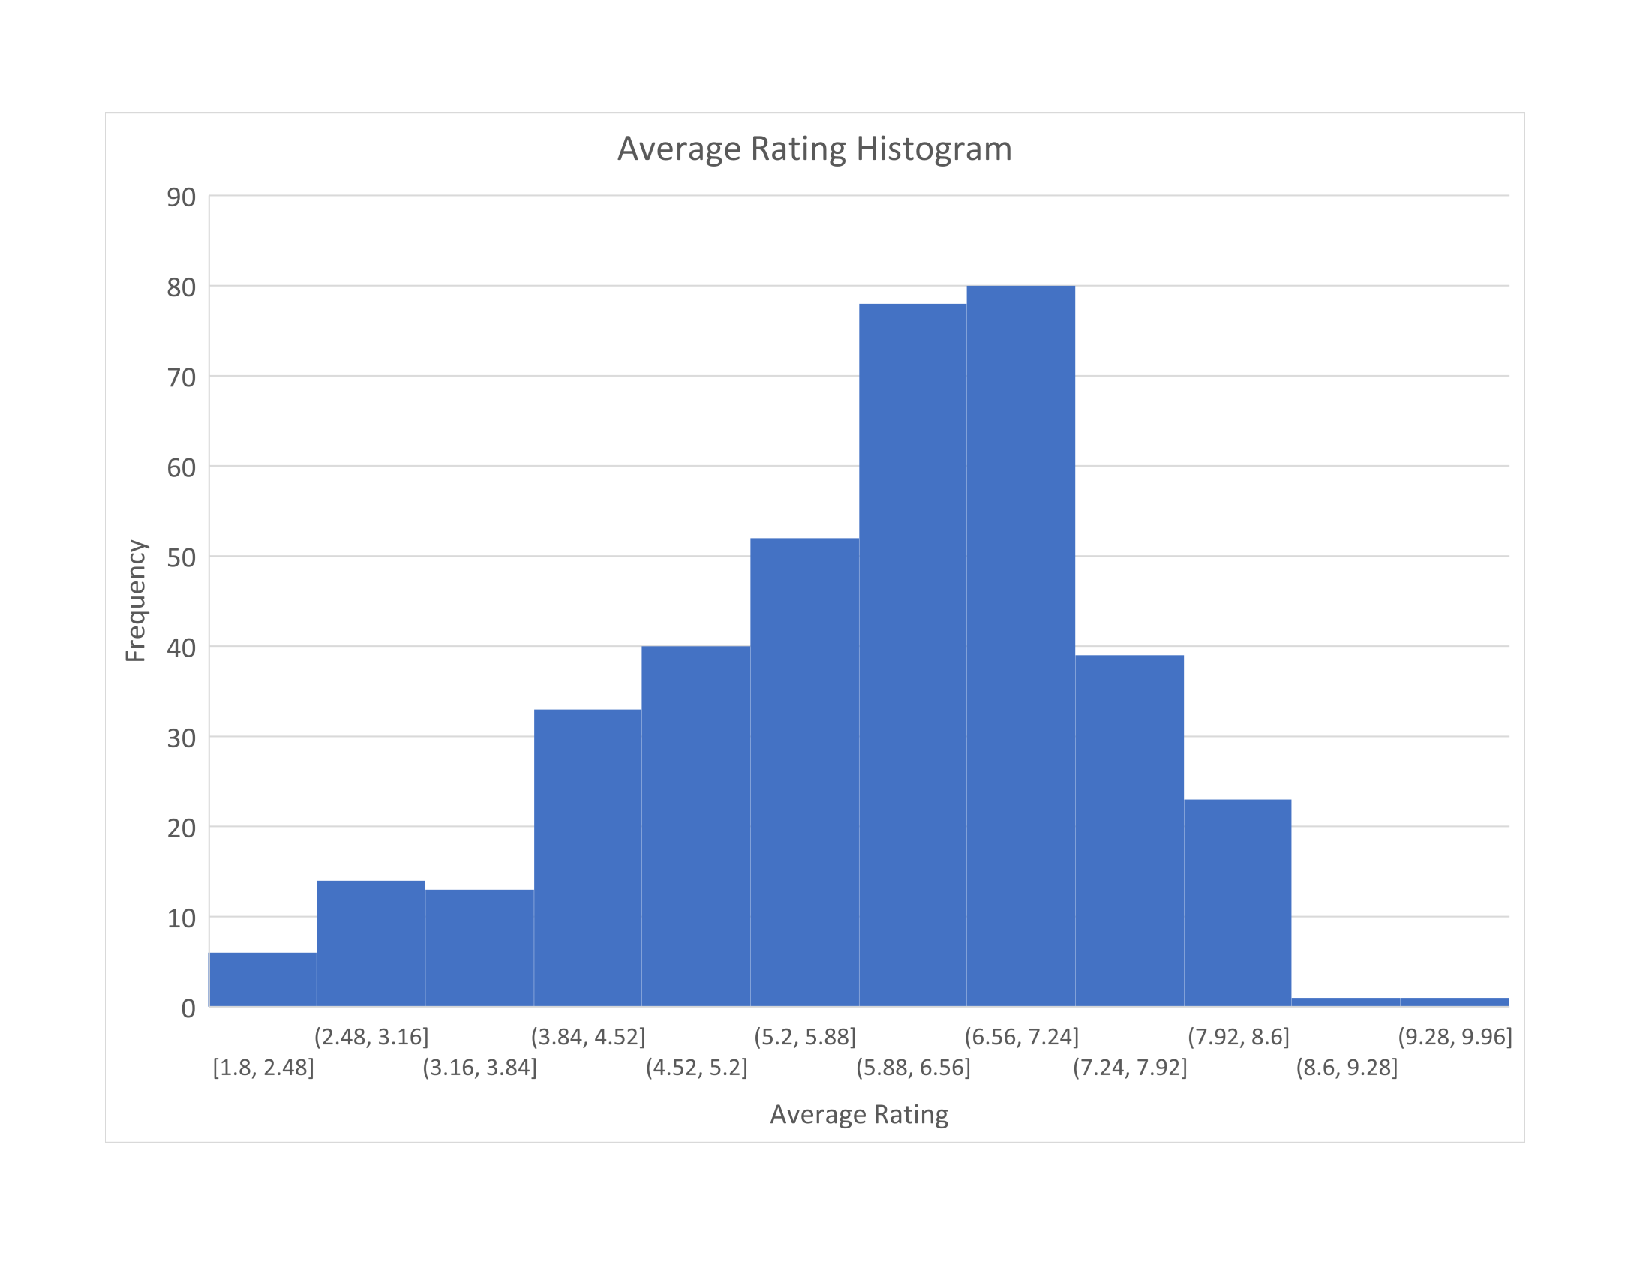
\includegraphics[clip, trim=0cm 2cm 0cm 2cm, width=1\textwidth]{averageRating_Histogram.pdf}  
    \caption{Figure {\color{franklinblue} 1}: Average Rating Histogram}
    \label{fig:arhist}
\end{figure}
\end{frame}

\begin{frame}[t]{Shapes of Histograms}
The following applies to frequency histograms and relative frequency histograms. \\
\vspace{1.5ex}
A histogram is \empr{skewed} if one side, or tail, is longer than the other. A histogram with a long right-hand tail is said to be \empr{skewed to the right}, or \empr{positively skewed}. A histogram with a long left-hand tail is said to be \empr{skewed to the left}, or \empr{negatively skewed}. \\
\vspace{1.5ex}
A histogram is \empr{symmetric} if its right half is a mirror image of its left half. Very few histograms are perfectly symmetric, but many are approximately symmetric. \\
\vspace{0ex}
\small 
\begin{itemize}
\item  A symmetric histogram with a peak in the middle is referred to as a \empr{bell-shaped histogram}.
\item A histogram in which all the classes have equal frequencies is said to be \empr{uniformly distributed}.
\end{itemize}
\end{frame}

\begin{frame}[t]{Mode}
A peak, or high point, of a histogram is referred to as a \empr{mode}.  The mode, if one exists, is thus the most frequently occurring value. \\
\vspace{1.5ex}
A histogram is \empr{unimodal} if it has only one mode, and \empr{bimodal} if it has two clearly distinct modes. \\
\vspace{1.5ex}
While some textbooks refer to the mode as a measure of \empr{central tendency}, I recommend \underline{not} using it as such. The mean and median are preferred measures of central tendency.
\end{frame}

\begin{frame}[t]{Misleading Histograms}
We know that the width of all histogram intervals, at times referred to as \empr{bins}, should be the same. \\
\vspace{1.5ex}
Suppose a data set contains many observations that fall into a relatively narrow part of the range, whereas others are widely dispersed. We might be tempted to construct a frequency distribution with narrow intervals where the bulk of the observations are and broader ones elsewhere. \\
\vspace{1.5ex}
Even if we remember that it is the areas, rather than the heights, of the rectangles of the histogram that must be proportional to the frequencies, it is still never a desirable option to construct such a histogram with different bin widths because it may easily deceive or distort the findings. We included this section simply to point out potential errors that we might find in histograms.
\end{frame}

\begin{frame}[t]{Creating the Central Tendency Table in Excel}
  Firstly, in your Excel workbook \texttt{IMDB\_BUSA\_603} create a sheet \texttt{Central\_Tendency} by clicking the 
\texttt{$\bigoplus$} at the bottom of the workbook.\footnote{All numerical summaries and illustrations presented in these lecture notes are available in the Excel workbook \texttt{IMDB\_BUSA\_603\_Module\_2}.}  \\
\vspace{1.5ex}
\begin{itemize}
\item In cell \texttt{A1} type \texttt{Measure}. In cell \texttt{B1} type {Category}.  In cell \texttt{C1} type \texttt{Value}.  For each typed value, place it in bold font. 
\item Then type entries for \texttt{Measures} and \texttt{Category} in cells \texttt{A2} through \texttt{B23} to produce Table \ref{tab:averageratingct} as illustrated above.
\end{itemize} 
\end{frame}

\begin{frame}[t]{Calculating in Excel Central Tendency Measures}
\small
 We will place the requested summary statistics in the tab \texttt{Central\_Tendency}.\\  
\begin{enumerate}
\item In cell \texttt{C2} type \texttt{=ROUND(AVERAGE(IMDB\_BUSA\_603!\$Q\$2:\$Q\$381),2)} to calculate the mean using all observations. By using the \texttt{ROUND} command we are maintaining 2 decimal points for the statistic.
\item In cell \texttt{C3} type \texttt{=ROUND(SUMPRODUCT(IMDB\_BUSA\_603!\$Q\$2:\$Q\$381, \\ IMDB\_BUSA\_603!\$R\$2:\$R\$381) \\ /SUM(IMDB\_BUSA\_603!\$R\$2:\$R\$381),2)} to calculate the weighted mean using all observations, where \texttt{numVotes} is the weight variable.  
\item In cell \texttt{C4} type \texttt{=ROUND(MEDIAN(IMDB\_BUSA\_603!\$Q\$2:\$Q\$381),2)} to calculate the median using all observations.
\item In cell \texttt{C5} type \texttt{=MODE.SNGL(IMDB\_BUSA\_603!\$Q\$2:\$Q\$381)} to calculate the mode using all observations.
\end{enumerate}
\end{frame}

\begin{frame}[t]{Calculating in Excel Group-Level Means \ldots}
\small
\begin{enumerate}
\setcounter{enumi}{4}
\item In cell \texttt{C6} type \texttt{=ROUND(AVERAGEIF(IMDB\_BUSA\_603!\$S\$2:\$S\$381,B6, \\ IMDB\_BUSA\_603!\$Q\$2:\$Q\$381),2)} to calculate the mean for \texttt{Comedy} observations. The cell value for \texttt{B6} of the formula resolves to \texttt{``Comedy''}.
\item In cell \texttt{C7} type \texttt{=ROUND(SUMPRODUCT(IF(IMDB\_BUSA\_603!\$S\$2:\$S\$381=B7, \\ IMDB\_BUSA\_603!\$Q\$2:\$Q\$381*IMDB\_BUSA\_603!\$R\$2:\$R\$381)) \\ /SUMIF(IMDB\_BUSA\_603!\$S\$2:\$S\$381,B7, \\ IMDB\_BUSA\_603!\$R\$2:\$R\$381),2)} to calculate the weighted mean for \texttt{Comedy} observations where \texttt{numVotes} is the weight variable.  
\item In cell \texttt{C8} type \texttt{=MEDIAN(IF(IMDB\_BUSA\_603!\$S\$2:\$S\$381=B8, \\ IMDB\_BUSA\_603!\$Q\$2:\$Q\$381))} to calculate the median for \texttt{Comedy} observations.
\item In cells \texttt{C9} through \texttt{C23} complete steps 5, 6, and 7 above for the other values of \texttt{Category} in the table. 
\end{enumerate}
\end{frame}

\begin{frame}[t]{Average Rating Central Tendency Measures}
%https://www.automateexcel.com/formulas/sumproduct-if/
% Table generated by Excel2LaTeX from sheet 'Central_Tendency'
\begin{table}[htbp]
  \centering
    \captionsetup{justification=centering}
    \begin{tabular}{llr}
    \rowcolor[rgb]{ .851,  .882,  .949} \textbf{Measure} & \textbf{Category} & \multicolumn{1}{l}{\textbf{Value}} \\
    Mean  & All   & 5.95 \\
    Weighted Mean & All   & 7.3 \\
    Median & All   & 6.1 \\
    Mode  & All   & 6 \\
    Mean  & Comedy & 6.03 \\
    Weighted Mean & Comedy & 7.18 \\
    Median & Comedy & 6.1 \\
    Mean  & Documentary & 7.27 \\
    Weighted Mean & Documentary & 7.44 \\
    Median & Documentary & 7.15 \\
    \end{tabular}%
  \label{tab:arctm1}%
\end{table}%
\end{frame}

\begin{frame}[t]{Average Rating Central Tendency Measures Cont.}
% Table generated by Excel2LaTeX from sheet 'Central_Tendency'
\begin{table}[htbp]
  \centering
  \captionsetup{justification=centering}
    \begin{tabular}{llr}
    \rowcolor[rgb]{ .851,  .882,  .949} \textbf{Measure} & \textbf{Category} & \multicolumn{1}{l}{\textbf{Value}} \\
    Mean  & Drama & 6.14 \\
    Weighted Mean & Drama & 7.69 \\
    Median & Drama & 6.3 \\
    Mean  & Horror & 4.74 \\
    Weighted Mean & Horror & 6.87 \\
    Median & Horror & 4.75 \\
    Mean  & Sci-Fi & 5.79 \\
    Weighted Mean & Sci-Fi & 7.33 \\
    Median & Sci-Fi & 6 \\
    Mean  & Other & 5.86 \\
    Weighted Mean & Other & 7.21 \\
    Median & Other & 5.7 \\
    \end{tabular}%
    \caption{Average Rating Central Tendency Measures}
  \label{tab:arctm2}%
\end{table}%
\vspace{-2.0ex}

\end{frame}

\begin{frame}[t]{Calculating in Excel Spread Measures}
 We will place the requested spread summary statistics in the tab \texttt{Spread}, where the tab is created in a manner analagous to that used to create \texttt{Central\_Tendency}.\\
\vspace{1.5ex}
Recall that the IMDb data is a \underline{sample} of the population of movies.  Thus we will calculate \underline{sample} measures of spread.\\
\small
\begin{enumerate}
\item In cell \texttt{C2} type \texttt{=ROUND(MAX(IMDB\_BUSA\_603!\$Q\$2:\$Q\$381)- \\ MIN(IMDB\_BUSA\_603!\$Q\$2:\$Q\$381),3)} to calculate the range using all observations. The invoked \texttt{ROUND} command means we are maintaining  3 decimal points for the statistic.  
\item In cell \texttt{C3} type \texttt{=ROUND(VAR.S(IMDB\_BUSA\_603!\$Q\$2:\$Q\$381),3)} to calculate the variance using all observations.  
\item In cell \texttt{C4} type \texttt{=ROUND(STDEV.S(IMDB\_215!\$Q\$2:\$Q\$381),3)} to calculate the standard deviation using all observations.  In lieu of this formula, one may have use \texttt{=ROUND(SQRT(C3),3)} to calculate the measure. 
\end{enumerate}
\end{frame}

\begin{frame}[t]{Calculating in Excel Group-Level Ranges \ldots}
\small
\begin{enumerate}
\setcounter{enumi}{3}
\item In cell \texttt{C5} type \texttt{=ROUND(MAXIFS(IMDB\_BUSA\_603!\$Q\$2:\$Q\$381, \\ IMDB\_BUSA\_603!\$S\$2:\$S\$381,B6)- \\ MINIFS(IMDB\_BUSA\_603!\$Q\$2:\$Q\$381, \\ IMDB\_BUSA\_603!\$S\$2:\$S\$381,B5),3)} to calculate the range for \texttt{Comedy} observations. The cell value for \texttt{B5} of the formula resolves to \texttt{``Comedy''}.
\item In cell \texttt{C6} type \texttt{=ROUND(((SUMPRODUCT(IF(IMDB\_BUSA\_603!\$S\$2:\$S\$381=B6,
IMDB\_BUSA\_603!\$Q\$2:\$Q\$381*IMDB\_BUSA\_603!\$Q\$2:\$Q\$381)))
-COUNTIF(IMDB\_BUSA\_603!\$S\$2:\$S\$381,B6)*AVERAGEIF(
IMDB\_BUSA\_603!\$S\$2:\$S\$381,B6,
IMDB\_BUSA\_603!\$Q\$2:\$Q\$381)$\hat{}\;2$)
/COUNTIF(IMDB\_BUSA\_603!\$S\$2:\$S\$381,B6),3)}
 to calculate the variance for \texttt{Comedy} observations.  
\item In cell \texttt{C7} type \texttt{=ROUND(SQRT(C6),3)} to calculate the standard deviation for \texttt{Comedy} observations.
\end{enumerate}
\end{frame}

\begin{frame}[t]{Average Rating Spread Measures}
% Table generated by Excel2LaTeX from sheet 'Central_Tendency'
% Table generated by Excel2LaTeX from sheet 'Spread'
\begin{enumerate}
  \setcounter{enumi}{6}
\item In cells \texttt{C8} through \texttt{C22} complete steps 4, 5, and 6 above for the other values of \texttt{Category} in the table. \\
\vspace{1.5ex}
\end{enumerate}
\begin{table}[htbp]
  \centering
    \captionsetup{justification=centering}
    \begin{tabular}{llr}
    \rowcolor[rgb]{ .851,  .882,  .949} \textbf{Measure} & \textbf{Category} & \multicolumn{1}{l}{\textbf{Value}} \\
    Range & All   & 7.6 \\
    Variance & All   & 1.991 \\
    Standard Deviation & All   & 1.411 \\
    Range & Comedy & 6.4 \\
    Variance & Comedy & 1.645 \\
    Standard Deviation & Comedy & 1.283 \\
    Range & Documentary & 2.4 \\
    Variance & Documentary & 0.469 \\
    Standard Deviation & Documentary & 0.685 \\
    \end{tabular}%
\end{table}%
\end{frame}

\begin{frame}[t]{Average Rating Spread Measures Continued}
% Table generated by Excel2LaTeX from sheet 'Spread'
\begin{table}[htbp]
  \centering
    \captionsetup{justification=centering}
    \begin{tabular}{llr}
    \rowcolor[rgb]{ .851,  .882,  .949} \textbf{Measure} & \textbf{Category} & \multicolumn{1}{l}{\textbf{Value}} \\
    Range & Drama & 6.7 \\
    Variance & Drama & 1.366 \\
    Standard Deviation & Drama & 1.169 \\
    Range & Horror & 5.8 \\
    Variance & Horror & 1.953 \\
    Standard Deviation & Horror & 1.397 \\
    Range & Sci-Fi & 6.2 \\
    Variance & Sci-Fi & 1.958 \\
    Standard Deviation & Sci-Fi & 1.399 \\
    Range & Other & 7.1 \\
    Variance & Other & 2.194 \\
    Standard Deviation & Other & 1.481 \\
    \end{tabular}%
  \caption{Average Rating Spread Measures} 
  \label{tab:addlabel}%
\end{table}%
\vspace{-2.0ex}

\end{frame}

\end{document}